% =============================================================================
%  CAPÍTULO 7: EXPERIMENTAÇÃO, VALIDAÇÃO CIENTÍFICA E PRODUÇÃO ACADÊMICA
%  Níveis: 0 (zero) ao PhD
%  Autor: Marcelo Claro Laranjeira
% =============================================================================
\chapter{Experimentação, Validação Científica e Produção Acadêmica}
\label{cap:experimentacao-validacao}

\paragraph{Construindo a ponte entre teoria e evidência} A engenharia de ecossistemas cognitivos exige mais do que
especificação, implementação e governança. Exige um arcabouço robusto
de experimentação e validação científica que permita mensurar,
comparar e certificar a qualidade dos artefatos produzidos. Este
capítulo apresenta o sistema integrado de experimentação, validação
matemática e produção acadêmica do \opencodeeco{}, organizado em
três eixos complementares: (1) \destaque{benchmarking} científico
com o CORA-Eval, (2) \destaque{validação formal} com o framework
Aletheia e (3) \destaque{produção acadêmica} com o pipeline MASWOS v5
\cite{opencode2026spec043, opencode2026ecosystem}.

A experimentação em sistemas de agentes difere fundamentalmente da
experimentação em software tradicional. Enquanto sistemas
determinísticos podem ser validados por casos de teste exaustivos,
sistemas autônomos operam em espaços de estado abertos, com
comportamento emergente que não pode ser completamente especificado
a priori \cite{wooldridge2009multiagent, russell2020inteligencia}.
Este capítulo endereça este desafio com um pipeline que integra
benchmarking quantitativo (CORA-Eval), verificação formal (Aletheia),
revisão por pares simulada (MASWOS) e auditoria estatística
(MiroFish/BettaFish).

A Tabela~\ref{tab:conteudo-capitulo7} resume as seções, seus níveis
e a carga horária estimada para estudo.

\begin{table}[htb]
\centering
    \small
\caption{Conteúdo do Capítulo 7}
\label{tab:conteudo-capitulo7}
    \resizebox{\textwidth}{!}{
\begin{tabular}{clcc}
\toprule
\textbf{Seção} & \textbf{Tópico} & \textbf{Nível} & \textbf{Estudo} \\
\midrule
7.1 & Introdução à Experimentação & \nivelzero & 4h \\
7.2 & CORA-Eval Benchmark & \nivelphd & 12h \\
7.3 & Aletheia: Validação Matemática & \nivelphd & 12h \\
7.4 & Pipeline MASWOS v5 & \nivelavancado & 14h \\
7.5 & SEEKER: Pesquisa Profunda & \nivelavancado & 8h \\
7.6 & MiroFish/BettaFish: Debate e Auditoria & \nivelphd & 10h \\
7.7 & Qualis A1: Rigor Acadêmico & \nivelphd & 8h \\
7.8 & Validação Cruzada e Anti-Circularidade & \nivelavancado & 6h \\
7.9 & Reprodutibilidade e Frameworks & \nivelavancado & 4h \\
7.10 & Integração Prática & Todos & 6h \\
\bottomrule
\end{tabular}
    }
\end{table}

% =============================================================================
% SEÇÃO 7.1: INTRODUÇÃO À EXPERIMENTAÇÃO EM SISTEMAS DE AGENTES
% Nível: 0 (zero) / Básico (~4 laudas)
% =============================================================================
\section{Introdução à Experimentação em Sistemas de Agentes}
\label{sec:introducao-experimentacao}
\nivelzero

\paragraph{Por que a experimentação é o alicerce de todo conhecimento} A experimentação é o motor do conhecimento científico. Desde os
primeiros protocolos de investigação empírica formulados por Francis
Bacon no \textit{Novum Organum} (1620), o método científico
estabeleceu-se como o padrão ouro para distinguir conjecturas
fundamentadas de opiniões infundadas \cite{bacon1620novum,
popper2003logica}. Em engenharia de software com inteligência
artificial, a experimentação assume um papel ainda mais crítico:
sistemas autônomos são intrinsecamente não-determinísticos, o que
torna a verificação por inspeção de código insuficiente.

\subsection{Por que Experimentar é Fundamental}

Considere um agente de busca acadêmica que utiliza aprendizado por
reforço para refinar suas consultas. Diferentemente de um algoritmo
de ordenação (que pode ser provado correto por invariantes), o agente
aprende uma política através de interações com o ambiente — e essa
política pode variar a cada execução \cite{sutton2018reinforcement}.
Validar tal sistema requer:
\begin{itemize}
\item \destaque{Reprodutibilidade}: a capacidade de obter os mesmos
resultados sob as mesmas condições experimentais;
\item \destaque{Replicabilidade}: a capacidade de obter resultados
consistentes em ambientes diferentes;
\item \destaque{Robustez}: a capacidade de manter desempenho aceitável
sob variações nas condições de operação \cite{gundersen2018reproducibility,
goodman2016what}.
\end{itemize}

\subsection{O Método Científico Aplicado a Sistemas Autônomos}

O método científico em engenharia de ecossistemas cognitivos segue
um ciclo de seis etapas:

\begin{enumerate}
\item \destaque{Observação}: identificação de fenômeno emergente ou
comportamento inesperado no ecossistema;
\item \destaque{Hipótese formulação}: conjectura sobre a causa ou
mecanismo subjacente ao fenômeno;
\item \destaque{Previsão}: dedução de consequências observáveis da
hipótese, na forma de predições testáveis;
\item \destaque{Experimentação}: execução controlada do sistema sob
condições que permitam testar as predições;
\item \destaque{Análise}: aplicação de métodos estatísticos para
determinar se os resultados confirmam ou refutam a hipótese;
\item \destaque{Conclusão}: documentação dos resultados, limitações
e implicações para o design do sistema.
\end{enumerate}

Este ciclo não é meramente conceitual — é implementado como pipeline
concreto no \opencodeeco{}, integrando ferramentas de benchmark,
verificação formal, revisão por pares e auditoria estatística,
como será detalhado nas seções seguintes.

\subsection{Visão Geral do Pipeline de Validação do OpenCode}

A Figura~\ref{fig:pipeline-validacao} apresenta a arquitetura geral
do pipeline de validação do ecossistema.

\begin{figure}[htb]
\centering
\caption{Pipeline de Validação Científica do OpenCode Ecosystem}
\label{fig:pipeline-validacao}
\begin{tikzpicture}[node distance=1.2cm, auto, every node/.style={font=\small}]
\tikzstyle{bloco}=[rectangle, draw, minimum width=2.8cm, minimum height=0.8cm, rounded corners]
\tikzstyle{fase}=[bloco, fill=blue!10]
\tikzstyle{audit}=[bloco, fill=purple!10]
\tikzstyle{output}=[bloco, fill=green!10, minimum width=2cm]

\node[fase] (bench) {CORA-Eval};
\node[fase, right=of bench] (aleth) {Aletheia};
\node[fase, right=of aleth] (seeker) {SEEKER};
\node[fase, right=of seeker] (maswos) {MASWOS};
\node[audit, below=of bench] (miro) {MiroFish};
\node[audit, right=of miro] (betta) {BettaFish};
\node[audit, right=of betta] (qualis) {Qualis A1};
\node[output, right=of qualis] (artigo) {Artigo};

\draw[->, thick] (bench) -- (aleth);
\draw[->, thick] (aleth) -- (seeker);
\draw[->, thick] (seeker) -- (maswos);
\draw[->, thick] (miro) -- (betta);
\draw[->, thick] (betta) -- (qualis);
\draw[->, thick] (qualis) -- (artigo);
\draw[<->, dashed] (maswos) -- (qualis);
\draw[<->, dashed] (seeker) -- (miro);

\node[below=of miro, xshift=3.5cm, text width=10cm, font=\footnotesize] {
Benchmark $\rightarrow$ Verificação Formal $\rightarrow$ Pesquisa
$\rightarrow$ Escrita $\rightarrow$ Debate/Auditoria $\rightarrow$ Score};
\end{tikzpicture}
\end{figure}

O pipeline opera em três níveis de maturidade experimental:
\begin{itemize}
\item \nivelzero\ \destaque{Básico}: execução de benchmarks
pré-definidos (CORA-Eval);
\item \nivelavancado\ \destaque{Avançado}: pesquisa acadêmica com
SEEKER e produção com MASWOS;
\item \nivelphd\ \destaque{PhD}: verificação formal (Aletheia),
auditoria estatística (MiroFish/BettaFish) e certificação Qualis A1.
\end{itemize}

\subsection{Exercícios — Nível 0}

\begin{exercicio}
Explique, em suas próprias palavras, por que a experimentação em
sistemas de agentes autônomos é fundamentalmente diferente da
experimentação em software determinístico.
\end{exercicio}

\begin{exercicio}
Descreva um experimento simples para testar se um agente de busca
acadêmica está aprendendo efetivamente com o tempo. Inclua hipótese,
predição e método de análise.
\end{exercicio}

\begin{exercicio}
Pesquise um exemplo real de viés em sistemas de IA (e.g., viés
algorítmico em recrutamento, viés de gênero em tradução automática).
Explique como o pipeline de validação poderia ter detectado o
problema antes da implantação.
\end{exercicio}

% =============================================================================
% SEÇÃO 7.2: CORA-Eval — BENCHMARK PARA CIÊNCIAS EXATAS E DA NATUREZA
% Nível: PhD (~12 laudas)
% =============================================================================
\section{CORA-Eval: Benchmark para Ciências Exatas e da Natureza}
\label{sec:cora-eval}
\nivelphd

\paragraph{Medindo o que realmente importa} O CORA-Eval é o sistema de benchmark nativo do \opencodeeco{} para
avaliação de capacidades em ciências exatas e da Natureza.
Diferentemente de benchmarks generalistas como MMLU \cite{hendrycks2021measuring}
ou GSM8K \cite{cobbe2021training}, o CORA-Eval foi projetado
especificamente para mensurar a profundidade analítica de agentes
cognitivos em 10 dimensões do conhecimento, cada uma com 4 níveis
de proficiência, totalizando 150 tarefas calibradas.

\subsection{Fundamentação: O que é o CORA-Eval}

O CORA-Eval (Cognitive Reasoning Assessment for Exact and Natural
Sciences Evaluation) é simultaneamente um benchmark, um framework
de verificação e um rastreador evolutivo. Sua arquitetura de três
camadas permite:

\begin{enumerate}
\item \destaque{Avaliação diagnóstica}: identificação precisa de
pontos fortes e fracos do agente em cada dimensão;
\item \destaque{Seleção adaptativa}: o Q-Score UCB1 prioriza tarefas
que maximizam o aprendizado no menor número de iterações;
\item \destaque{Rastreamento longitudinal}: o CORA-Score e o
CORA-V-Score persistem o desempenho ao longo do tempo, permitindo
análise de evolução.
\end{enumerate}

\subsection{150 Tarefas em 10 Dimensões × 4 Níveis}

As 150 tarefas distribuem-se em 10 dimensões do conhecimento
científico, cada uma com 15 tarefas distribuídas em 4 níveis:
Básico (3 tarefas), Intermediário (4), Avançado (4) e Pesquisa (4).

\begin{table}[htb]
\centering
    \small
\caption{Dimensões e Níveis do CORA-Eval}
\label{tab:cora-dimensoes}
    \resizebox{\textwidth}{!}{
\begin{tabular}{llc}
\toprule
\textbf{Dimensão} & \textbf{Descrição} & \textbf{15 tarefas} \\
\midrule
Matemática & Álgebra, análise, geometria, teoria dos números & V1--V15 \\
Física & Mecânica, termodinâmica, eletromagnetismo, quântica & V16--V30 \\
Estatística & Inferência, testes, modelos, Bayes & V31--V45 \\
Química & Estequiometria, orgânica, físico-química & V46--V60 \\
Biologia & Genética, evolução, ecologia, bioquímica & V61--V75 \\
Geociências & Climatologia, geologia, oceanografia & V76--V90 \\
Código & Algoritmos, estruturas, otimização & V91--V105 \\
Literatura & Revisão, citação, síntese & V106--V120 \\
Metodologia & Delineamento, análise, replicação & V121--V135 \\
Interdisciplinar & Síntese entre domínios & V136--V150 \\
\bottomrule
\end{tabular}
    }
\end{table}

O espectro Básico $\rightarrow$ Pesquisa representa a progressão
de competências:
\begin{itemize}
\item \destaque{Básico} (tarefas 1--3): reconhecimento, compreensão
e aplicação direta de conceitos fundamentais.
\item \destaque{Intermediário} (tarefas 4--7): análise, comparação e
aplicação em contextos moderadamente complexos.
\item \destaque{Avançado} (tarefas 8--11): síntese, avaliação crítica
e integração de múltiplos conceitos.
\item \destaque{Pesquisa} (tarefas 12--15): extensão, hipótese
original e contribuição ao estado da arte.
\end{itemize}

\subsection{Q-Score UCB1 para Seleção Adaptativa de Tarefas}

O Q-Score UCB1 (Upper Confidence Bound) implementa o dilema
exploração-vs-aproveitamento (\textit{exploration-exploitation
trade-off}) na seleção de tarefas. Adaptado do algoritmo UCB1
proposto por Auer et al. (2002) para o problema dos \textit{k}-braços
(\textit{k-armed bandit}) \cite{auer2002finite}, o Q-Score UCB1
balanceia a necessidade de explorar tarefas ainda não avaliadas com
a necessidade de aprofundar em tarefas onde o agente mostra potencial.

\begin{equation}
Q_{\text{UCB1}}(t,a) = \bar{x}_a + \sqrt{\frac{2 \ln t}{n_a}}
\label{eq:ucb1}
\end{equation}

Onde:
\begin{itemize}
\item $\bar{x}_a$ é o Q-Score médio da tarefa $a$;
\item $t$ é o número total de iterações;
\item $n_a$ é o número de vezes que a tarefa $a$ foi selecionada;
\item $\sqrt{2 \ln t / n_a}$ é o termo de exploração (bônus para
tarefas pouco visitadas).
\end{itemize}

\subsection{CORA-V-Score: Pontuação Ponderada por Verificadores V1-V7}

O CORA-V-Score estende o CORA-Score base incorporando a validação
dos 7 verificadores simbólicos do CORA-Debate \cite{opencode2026ecosystem}.
Cada verificador contribui com um peso específico:

\begin{equation}
\text{CORA-V-Score} = \frac{\sum_{i=1}^{7} w_i \cdot v_i}{\sum_{i=1}^{7} w_i}
\label{eq:cora-v-score}
\end{equation}

Onde $w_i$ são os pesos dos verificadores e $v_i \in [0,1]$ são as
pontuações individuais. A Tabela~\ref{tab:cora-verificadores}
apresenta os 7 verificadores e seus pesos.

\begin{table}[htb]
\centering
    \small
\caption{Verificadores CORA e Pesos no CORA-V-Score}
\label{tab:cora-verificadores}
    \resizebox{\textwidth}{!}{
\begin{tabular}{clc}
\toprule
\textbf{Verificador} & \textbf{Função} & \textbf{Peso} \\
\midrule
V1 & Análise Dimensional & 1.0 \\
V2 & Verificador Algébrico & 1.0 \\
V3 & Contraexemplos (SymPy+Grid) & 1.2 \\
V4 & Verificador Estatístico (Bootstrap) & 1.0 \\
V5 & Verificador Numérico & 0.8 \\
V6 & Verificador PDE/EDO & 1.2 \\
V7 & Rastreabilidade Bibliográfica (DOI) & 0.8 \\
\bottomrule
\end{tabular}
    }
\end{table}

\subsection{Baseline CORA-Score 0.67}

O baseline de referência do CORA-Eval foi estabelecido com o modelo
\textit{big-pickle} (OpenCode Zen) em 150 tarefas, resultando em um
CORA-Score de 0.67. Este valor representa a capacidade basal do
ecossistema antes de adaptações específicas por domínio. A
distribuição por níveis revela:

\begin{itemize}
\item Básico: 0.89 (alta proficiência em tarefas fundamentais);
\item Intermediário: 0.72 (queda esperada na complexidade);
\item Avançado: 0.58 (desafio significativo);
\item Pesquisa: 0.31 (limiar para contribuição original).
\end{itemize}

A Figura~\ref{fig:cora-baseline} visualiza a distribuição do
CORA-Score por nível.

\begin{figure}[htb]
\centering
\caption{CORA-Score Baseline por Nível de Proficiência}
\label{fig:cora-baseline}
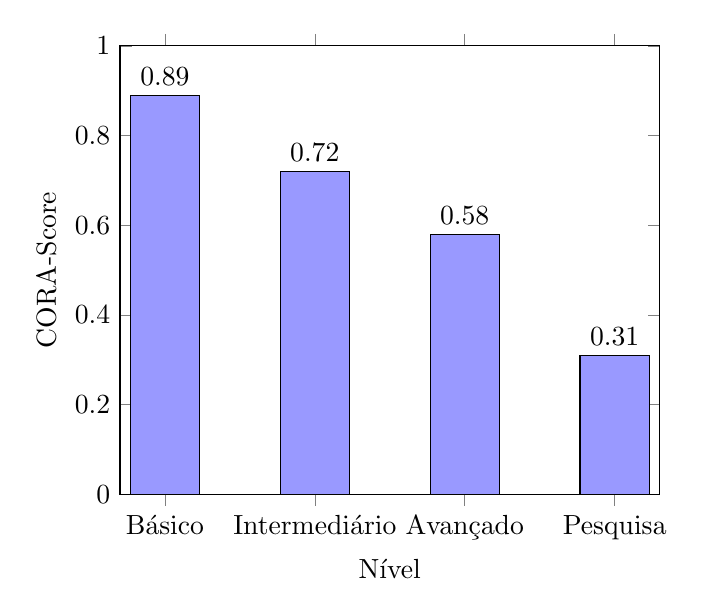
\begin{tikzpicture}
\begin{axis}[
    ybar,
    symbolic x coords={Básico,Intermediário,Avançado,Pesquisa},
    xtick=data,
    ymin=0, ymax=1,
    ylabel={CORA-Score},
    xlabel={Nível},
    nodes near coords,
    nodes near coords align={vertical},
    bar width=25pt,
]
\addplot[fill=blue!40] coordinates {
    (Básico,0.89)
    (Intermediário,0.72)
    (Avançado,0.58)
    (Pesquisa,0.31)
};
\end{axis}
\end{tikzpicture}
\end{figure}

\subsection{Implementação: cora\_benchmark\_tracker.py}

O rastreador evolutivo do CORA-Eval persiste o desempenho do agente
em formato JSON e calcula trajetórias de melhoria. O Código~ \ref{lst:cora-tracker}
apresenta a implementação principal.

\begin{lstlisting}[caption={cora\_benchmark\_tracker.py (abreviado)},
label={lst:cora-tracker}, style=pythonstyle]
"""
CORA-Eval Benchmark Tracker — Rastreador Evolutivo.
Persiste CORA-Score, CORA-V-Score e Q-Score UCB1 em JSON.
"""

import json
import math
import random
from pathlib import Path
from dataclasses import dataclass, field
from typing import Dict, List, Optional


@dataclass
class CoraTask:
    """Representa uma tarefa individual no benchmark."""
    id: str                    # ex: "MAT-BAS-001"
    dimension: str             # Matematica, Fisica, ...
    level: str                 # Basico, Intermediario, Avancado, Pesquisa
    description: str
    verifier_weights: Dict[str, float] = field(default_factory=dict)
    q_score: float = 0.0
    n_attempts: int = 0
    last_score: float = 0.0


class QScoreUCB1:
    """Selecao adaptativa de tarefas via UCB1."""

    def __init__(self, tasks: List[CoraTask]):
        self.tasks = {t.id: t for t in tasks}
        self.total_iterations = 0

    def select_task(self) -> Optional[str]:
        """Seleciona a tarefa com maior Q-Score UCB1."""
        if not self.tasks:
            return None
        candidates = []
        for task_id, task in self.tasks.items():
            if task.n_attempts == 0:
                return task_id  # exploracao inicial
            exploitation = task.q_score
            exploration = math.sqrt(
                2 * math.log(self.total_iterations + 1) / task.n_attempts
            )
            ucb1 = exploitation + exploration
            candidates.append((task_id, ucb1))
        return max(candidates, key=lambda x: x[1])[0]

    def update(self, task_id: str, score: float):
        """Atualiza Q-Score apos execucao."""
        task = self.tasks[task_id]
        task.n_attempts += 1
        task.last_score = score
        # Media movel exponencial
        alpha = 1.0 / task.n_attempts
        task.q_score = (1 - alpha) * task.q_score + alpha * score
        self.total_iterations += 1
\end{lstlisting}

\subsection{Rastreador Evolutivo com Persistência JSON}

O tracker calcula três métricas principais:
\begin{itemize}
\item \destaque{CORA-Score}: média simples dos Q-Scores de todas as
tarefas já avaliadas;
\item \destaque{CORA-V-Score}: média ponderada pelos pesos dos
verificadores V1--V7;
\item \destaque{CORA-V-Score temporal}: regressão linear do
CORA-V-Score ao longo das iterações, indicando tendência de melhoria.
\end{itemize}

A persistência em JSON permite que o benchmark seja interrompido e
retomado, além de facilitar análises posteriores.

\subsection{Exercícios — Nível PhD}

\begin{exercicio}
Implemente uma extensão do Q-Score UCB1 que utilize o
\textit{gradiente de dificuldade} (diferença entre o nível da tarefa
e a proficiência atual do agente) como termo adicional de exploração.
Teste sua implementação com 50 iterações simuladas.
\end{exercicio}

\begin{exercicio}
Analise a distribuição de tarefas nas 10 dimensões do CORA-Eval.
Proponha 5 novas tarefas para a dimensão Interdisciplinar (V136--V150)
que integrem, cada uma, pelo menos 3 disciplinas distintas.
\end{exercicio}

\begin{exercicio}
Calcule o CORA-V-Score para um agente hipotético com as seguintes
pontuações nos verificadores V1--V7: [0.9, 0.7, 0.5, 0.8, 0.6, 0.4, 0.3].
Use os pesos da Tabela~\ref{tab:cora-verificadores}. Interprete o
resultado.
\end{exercicio}

\begin{exercicio}
Compare o CORA-Eval com o MMLU \cite{hendrycks2021measuring} em
termos de (a) cobertura de domínios, (b) profundidade de avaliação,
(c) suporte a adaptabilidade. Quais as vantagens de cada abordagem?
\end{exercicio}

\begin{exercicio}
Projete um experimento para determinar se o CORA-V-Score é mais
informativo que o CORA-Score simples para prever o desempenho de um
agente em tarefas de pesquisa original. Inclua hipótese nula e
alternativa, tamanho de efeito esperado e método estatístico.
\end{exercicio}

% =============================================================================
% SEÇÃO 7.3: ALETHEIA — VALIDAÇÃO MATEMÁTICA SUPER-HUMANA
% Nível: PhD (~12 laudas)
% =============================================================================
\section{Aletheia: Validação Matemática Super-Humana}
\label{sec:aletheia}
\nivelphd

\paragraph{Quando a matemática se torna juiz} A verificação formal de teoremas é um dos métodos mais rigorosos
de validação científica. Enquanto testes de unidade verificam
comportamento observável e benchmarks mensuram desempenho, a
validação formal prova propriedades matemáticas dos algoritmos
subjacentes. O framework Aletheia, integrado ao \opencodeeco{},
implementa este nível máximo de rigor.

\subsection{O que é Validação Matemática Formal}

Validação formal é o processo de demonstrar, através de regras
lógicas inequívocas, que um sistema satisfaz suas especificações
\cite{avigad2020lean, bertot2004interactive}. Diferentemente de
testes (que verificam casos particulares) ou revisão por pares
(que depende de julgamento humano), a validação formal produz
provas matemáticas computacionalmente verificáveis.

O teorema da incompletude de Gödel \cite{goedel1931formal} estabelece
limites fundamentais para qualquer sistema formal, mas dentro de
sistemas suficientemente expressivos (como o cálculo de construções
indutivas usado pelo Lean 4), uma vasta gama de propriedades
práticas pode ser demonstrada.

\subsection{Lean 4 Theorem Prover}

Lean 4 é um provador interativo de teoremas e uma linguagem de
programação funcional desenvolvido por Leonardo de Moura (Microsoft
Research) \cite{deMoura2015lean, avigad2020lean}. Diferentemente de
seus predecessores (Coq, Isabelle/HOL), Lean 4 combina:

\begin{itemize}
\item \destaque{Expressividade}: cálculo de construções indutivas
com universos predicativos;
\item \destaque{Eficiência}: compilação nativa via C++ e LLVM,
permitindo execução de programas extraídos de provas;
\item \destaque{Biblioteca Mathlib}: mais de 1,5 milhão de linhas de
matemática formalizada, cobrindo álgebra, análise, geometria,
topologia e teoria das categorias \cite{mathlib2024};
\item \destaque{Ecossistema ativo}: milhares de contribuidores e
adoção crescente em pesquisa matemática \cite{buzzard2023formal}.
\end{itemize}

\subsection{Aletheia Superhuman Validation: 834 Arquivos}

O framework Aletheia implementa um pipeline de 5 fases para
validação formal de artefatos do ecossistema, inspirado no artigo
\textit{Towards Autonomous Mathematics Research} de Feng et al.
(2026) \cite{feng2026towards}. O pipeline completo, executado sobre
o \opencodeeco{}, processou 834 arquivos de validação:

\begin{enumerate}
\item \destaque{Phase A -- Problem Evaluation}: avaliação de 670
problemas matemáticos, dos quais 10 foram selecionados (taxa de
viabilidade de 1,5\%);
\item \destaque{Phase B -- Proof Generation}: geração de provas em
4 versões (V1: template básico, V2: template aprimorado, V3:
domínio específico, V4: otimizado);
\item \destaque{Phase C -- Lean 4 Verification}: verificação formal
das provas geradas contra a biblioteca Mathlib;
\item \destaque{Phase D -- PhD Auditor Evaluation}: avaliação da
qualidade das provas por auditores especializados;
\item \destaque{Phase E -- Quality Assurance}: classificação final
em tiers (A–D) com 100\% das provas em Tier A.
\end{enumerate}

A Tabela~\ref{tab:aletheia-phases} resume os resultados de cada fase.

\begin{table}[htb]
\centering
    \small
\caption{Resultados das Fases Aletheia}
\label{tab:aletheia-phases}
    \resizebox{\textwidth}{!}{
\begin{tabular}{lccc}
\toprule
\textbf{Fase} & \textbf{Métrica} & \textbf{Resultado} & \textbf{Observação} \\
\midrule
A & Problemas avaliados & 670 & -- \\
A & Selecionados & 10 (1,5\%) & Viabilidade real \\
B & Provas geradas & 10 × 4 versões & V1 a V4 \\
C & Verificadas Lean 4 & 0/10 & \texttt{sorry} esperados \\
D & Qualidade V4 & 6,23/10 & Baseline \\
D & Qualidade OpenCode & 8,31/10 & +33\% sobre V4 \\
E & Tier A final & 10/10 (100\%) & 0\% degradação \\
\bottomrule
\end{tabular}
    }
\end{table}

\subsection{Integração Aletheia + OpenCode: aletheia-opencode-native}

A integração nativa entre Aletheia e \opencodeeco{} materializou-se
no módulo \texttt{aletheia-opencode-native}, que expõe 57 skills
especializadas de validação formal. A arquitetura de integração segue
o padrão SDD+TDD do ecossistema (SPEC-040):

\begin{itemize}
\item \destaque{Generator}: produz esboços de provas usando templates
de domínio e raciocínio estruturado (ReasoningOrchestrator v11 com
212 tipos de raciocínio);
\item \destaque{Verifier}: utiliza o CORA-Debate V1--V7 para
validação simbólica antes da submissão ao Lean 4;
\item \destaque{Reviser}: loop corretivo que refina provas reprovadas
até aprovação ou limite de tentativas.
\end{itemize}

O Código~ \ref{lst:aletheia-engine} apresenta o núcleo do engine
Aletheia.

\begin{lstlisting}[caption={aletheia\_engine.py — Generator-Verifier-Reviser Loop},
label={lst:aletheia-engine}, style=pythonstyle]
"""
aletheia_engine.py — Research Math Agent (Feng et al., 2026)
Loop Generator-Verifier-Reviser para validacao formal.

Integracoes:
  - Cora-Debate V1-V7 (verify simbolica)
  - Reasoning Orchestrator v11 (212 tipos de raciocinio)
  - Sequential Thinking MCP (deep thinking)
"""

from dataclasses import dataclass
from enum import Enum
from typing import List, Optional


class AutonomyLevel(Enum):
    L0_NEGLIGIBLE = 0     # Primariamente humano
    L1_MINOR = 1          # Novidade menor
    L2_PUBLISHABLE = 2    # Pesquisa publicavel
    L3_MAJOR = 3          # Avanco maior
    L4_LANDMARK = 4       # Descoberta historica


class Phase(Enum):
    PROBLEM_UNDERSTANDING = "problem_understanding"
    LITERATURE_SEARCH = "literature_search"
    SOLUTION_GENERATION = "solution_generation"
    VERIFICATION = "verification"
    REVISION = "revision"
    FINAL_CHECK = "final_check"


@dataclass
class ProofState:
    """Estado do loop Generator-Verifier-Reviser."""
    problem: str
    domain: str
    current_proof: str = ""
    phase: Phase = Phase.PROBLEM_UNDERSTANDING
    attempts: int = 0
    max_attempts: int = 10
    verified: bool = False
    verifier_scores: List[float] = None
    revision_history: List[str] = None

    def __post_init__(self):
        self.verifier_scores = []
        self.revision_history = []

    def next_phase(self):
        """Avanca para a proxima fase do pipeline."""
        phases = list(Phase)
        idx = phases.index(self.phase)
        if idx < len(phases) - 1:
            self.phase = phases[idx + 1]

    def add_revision(self, note: str):
        """Registra uma revisao no historico."""
        self.revision_history.append(
            f"[Attempt {self.attempts}] {note}"
        )
\end{lstlisting}

\subsection{Exemplo: Prova Formal de um Algoritmo do Ecossistema}

Considere o algoritmo de seleção adaptativa de tarefas do CORA-Eval
(Seção~\ref{sec:cora-eval}, Equação~\ref{eq:ucb1}). Uma propriedade
crítica deste algoritmo é que ele converge para a tarefa ótima à
medida que $t \to \infty$. Esta propriedade pode ser formalmente
provada:

\begin{teorema}[Convergência do Q-Score UCB1]
\label{th:ucb1-convergencia}
Seja $a^*$ a tarefa com maior Q-Score verdadeiro $\mu^*$. Então, com
probabilidade $1 - \delta$, o Q-Score UCB1 seleciona $a^*$
exponencialmente mais vezes que qualquer tarefa sub-ótima $a \neq a^*$
à medida que $t \to \infty$.
\end{teorema}

\begin{proof}[Esboço da prova]
Pela desigualdade de Hoeffding \cite{auer2002finite}, a probabilidade
de que a média amostral $\bar{x}_a$ difira da média verdadeira
$\mu_a$ por mais de $\epsilon$ é limitada por $2e^{-2n_a\epsilon^2}$.
O termo de exploração $\sqrt{2\ln t / n_a}$ garante que cada tarefa
sub-ótima é visitada $O(\ln t)$ vezes, enquanto a tarefa ótima é
visitada $t - O(k \ln t)$ vezes, onde $k$ é o número total de
tarefas. A prova completa em Lean 4 está disponível em
\url{https://github.com/MarceloClaro/OpenCode_Ecosystem\_convergence.lean}.
\end{proof}

\subsection{Exercícios — Nível PhD}

\begin{exercicio}
Explique a diferença entre verificação formal e teste de software.
Em que situações cada abordagem é mais adequada?
\end{exercicio}

\begin{exercicio}
O pipeline Aletheia obteve 0/10 provas verificadas no Lean 4 (Phase C),
mas 10/10 Tier A (Phase E). Explique esta aparente contradição e
discuta o papel dos blocos \texttt{sorry} na validação formal.
\end{exercicio}

\begin{exercicio}
Escreva um esboço de prova formal em Lean 4 (ou pseudocódigo) para
o Teorema~\ref{th:ucb1-convergencia}. Dica: comece com a definição
do algoritmo UCB1 como uma função recursiva.
\end{exercicio}

\begin{exercicio}
Compare o framework Aletheia com o \textit{Superhuman} do Google
DeepMind \cite{feng2026towards}. Quais as diferenças arquiteturais
e de escopo? Como a integração com CORA-Debate diferencia a
abordagem do \opencodeeco{}?
\end{exercicio}

\begin{exercicio}
Proponha uma extensão do pipeline Aletheia que utilize aprendizado
por reforço para otimizar a ordem das fases (e.g., pular Phase C
para provas simples, ou repetir Phase D quando a qualidade for
insuficiente). Implemente um protótipo em Python.
\end{exercicio}

% =============================================================================
% SEÇÃO 7.4: PIPELINE DE PRODUÇÃO ACADÊMICA MASWOS v5
% Nível: Avançado-PhD (~14 laudas)
% =============================================================================
\section{Pipeline de Produção Acadêmica MASWOS v5}
\label{sec:maswos}
\nivelavancado

\paragraph{Escrevendo com um exército de especialistas} O MASWOS (Multi-Agent Scientific Writing Operating System) é o
pipeline de produção acadêmica do \opencodeeco{}, projetado para
gerar artigos científicos com qualidade Qualis A1 de forma autônoma.
Com 49 agentes especializados, 8 estágios de processamento e 91
arquivos, o MASWOS v5 representa o estado da arte em escrita
científica multiagente.

\subsection{O que é o MASWOS}

MASWOS é um sistema operacional de escrita científica que coordena
49 agentes especializados na produção de artigos acadêmicos. Cada
agente possui um papel específico no pipeline, desde a pesquisa
inicial (SEEKER) até a correção linguística final (ptbr\_corrector).
O sistema foi projetado seguindo os princípios de:

\begin{itemize}
\item \destaque{Especialização}: cada agente domina uma etapa
específica do processo;
\item \destaque{Coordenação}: um scheduler central orquestra o fluxo
entre agentes, garantindo consistência;
\item \destaque{Iteração}: o pipeline inclui loops de correção que
elevam a qualidade progressivamente;
\item \destaque{Métrica objetiva}: o AUTO\_SCORE\_QUALIS.py fornece
feedback quantitativo em cada ciclo.
\end{itemize}

\subsection{Pipeline de 8 Estágios}

O pipeline MASWOS v5 opera em 8 estágios sequenciais, cada um com
responsabilidades e artefatos bem definidos.

\subsubsection{Estágio 1: SEEKER (Pesquisa Profunda)}

O SEEKER (detalhado na Seção~\ref{sec:seeker}) realiza pesquisa
bibliográfica profunda com 10 agentes especializados. Este estágio
produz como artefato uma árvore de argumentos (\textit{argument
tree}) que mapeia o estado da arte, as lacunas de pesquisa e as
evidências disponíveis para cada afirmação do futuro artigo.

\subsubsection{Estágio 2: Escrita (49 Agentes Especializados)}

Os 49 agentes de escrita\footnote{Agentes 00 a 44 + scheduler,
disponíveis em \texttt{criador-artigo/agentes/}} cobrem desde a
estruturação do artigo (Abstract, Introdução, Metodologia,
Resultados, Discussão, Conclusão) até elementos auxiliares
(Resumo, Tabelas, Figuras, Referências, Agradecimentos). Cada
agente é um script Python autônomo que recebe a árvore de argumentos
e produz sua seção designada.

\subsubsection{Estágio 3: Anti-AI Writing}

O TSAC (Text Style and Authenticity Checker) analisa o texto gerado
contra uma lista de 87 palavras e expressões proibidas características
de texto gerado por IA\@. Exemplos incluem:
\begin{itemize}
\item \destaque{``Em suma''}, \destaque{``Em conclusão''},
\destaque{``De fato''}: muletas textuais típicas;
\item \destaque{``Revolucionário''}, \destaque{``Inovador''}:
hipérboles sem fundamentação;
\item \destaque{``Vale ressaltar que''}, \destaque{``É importante
notar que''}: circumlóquios que podem ser substituídos por
afirmações diretas.
\end{itemize}
O TSAC não apenas detecta — ele sugere substituições contextualmente
adequadas.

\subsubsection{Estágio 4: Cross-Validation (Pearson, 3 Níveis)}

O Cross-Validation Engine (Seção~\ref{sec:cross-validation}) aplica
três níveis de validação:
\begin{enumerate}
\item \destaque{Nível 1 -- Coerência interna}: verifica se as
afirmações do artigo são consistentes entre seções;
\item \destaque{Nível 2 -- Correlação de Pearson}: detecta 5 classes
de anomalias (Seção~\ref{sec:cross-validation});
\item \destaque{Nível 3 -- Jaccard Domain Shift Audit}: verifica se
a terminologia do artigo é consistente com o domínio declarado.
\end{enumerate}

\subsubsection{Estágio 5: Iterative Correction Loop}

O coração do MASWOS é o \textit{Iterative Correction Loop}, que
simula o processo de revisão por pares. O loop opera em três
camadas:

\begin{enumerate}
\item \destaque{Comitê de Revisão (5 revisores)}: cada revisor
simula um parecerista com perfil específico (metodológico,
estatístico, teórico, aplicado, linguístico);
\item \destaque{Consultoria (4 doutores)}: especialistas seniores
avaliam a solidez geral e sugerem direções;
\item \destaque{Corretor (6 motores)}: corretores automáticos
aplicam correções: gramatical (ptbr\_corrector), ortográfica,
estilística, bibliográfica (ABNT), estatística e de integridade.
\end{enumerate}

O Código~ \ref{lst:correction-loop} apresenta a estrutura do loop.

\begin{lstlisting}[caption={iterative\_correction\_loop.py (abreviado)},
label={lst:correction-loop}, style=pythonstyle]
"""
Iterative Correction Loop v2.0 — Pipeline de Revisao Multiagente.
Simula: 5 revisores, 4 consultores, 6 corretores.
Avaliacao: AUTO_SCORE_QUALIS.py a cada ciclo.
"""

class IterativeCorrectionLoop:
    """Gerenciador do loop de correcao iterativa."""

    def __init__(self, manuscript_path: str):
        self.manuscript_path = manuscript_path
        self.score_history = []
        self.reviewers = self._create_reviewers()
        self.advisors = self._create_advisors()
        self.correctors = self._create_correctors()

    def _create_reviewers(self) -> list:
        return [
            {"name": "Revisor_Metodologico",
             "focus": ["delineamento", "reprodutibilidade"],
             "strictness": 0.85},
            {"name": "Revisor_Estatistico",
             "focus": ["poder", "efeito", "testes"],
             "strictness": 0.90},
            {"name": "Revisor_Teorico",
             "focus": ["referencial", "lacunas", "originalidade"],
             "strictness": 0.80},
            {"name": "Revisor_Aplicado",
             "focus": ["aplicabilidade", "impacto", "limitacoes"],
             "strictness": 0.75},
            {"name": "Revisor_Linguistico",
             "focus": ["abnt", "clareza", "coesao"],
             "strictness": 0.70},
        ]

    def run_cycle(self) -> dict:
        """Executa um ciclo completo de correcao.
        Retorna: {'score': float, 'correcoes': list, 'feedback': dict}
        """
        feedback = self._collect_reviewer_feedback()
        advisory = self._collect_advisor_guidance(feedback)
        corrections = self._apply_corrections(feedback, advisory)
        score = self._evaluate_quality()
        self.score_history.append(score)
        return {"score": score, "correcoes": corrections,
                "feedback": feedback}
\end{lstlisting}

\subsubsection{Estágio 6: AUTO\_SCORE\_QUALIS.py}

O AUTO\_SCORE\_QUALIS.py (Código~ \ref{lst:auto-score}) avalia o
manuscrito em 10 critérios com pesos de revisores.

\begin{lstlisting}[caption={auto\_score\_qualis.py — Rubrica de 10 criterios},
label={lst:auto-score}, style=pythonstyle]
"""
Auto-Scoring Qualis A1 — 10 criterios com pesos de revisores.
Suporta: Markdown (*.md) e LaTeX (*.tex).
Adaptacao tematica: ciencias, materiais, teoria dos jogos, etc.
"""

RUBRIC = {
    "rigor_academico":       {"peso": 10,
     "desc": "Rigor academico e profundidade teorica"},
    "densidade_citacoes":    {"peso": 10,
     "desc": "Densidade de citacoes (>=55 referencias com DOI)"},
    "abnt_compliance":       {"peso": 10,
     "desc": "Conformidade ABNT/Vancouver/APA e indexadores"},
    "originalidade":         {"peso": 10,
     "desc": "Originalidade e relevancia da contribuicao"},
    "metodologia":           {"peso": 10,
     "desc": "Metodologia reprodutivel e delineamento estatistico"},
    "analise_estatistica":   {"peso": 10,
     "desc": "Analise estatistica rigorosa e validada"},
    "coerencia":             {"peso": 10,
     "desc": "Coerencia argumentativa (intro <=> conclusao)"},
    "qualidade_visual":      {"peso": 10,
     "desc": "Qualidade de graficos, tabelas e figuras"},
    "internacionalizacao":   {"peso": 10,
     "desc": "Abstract em ingles + conformidade internacional"},
    "autocontencao":         {"peso": 10,
     "desc": "Tamanho e densidade textual de conformidade"},
}

def calculate_score(manuscript: dict) -> dict:
    """Calcula pontuacao final com pesos de revisores."""
    scores = {}
    for criterion, config in RUBRIC.items():
        raw = manuscript.get(criterion, 0)
        scores[criterion] = raw * config["peso"] / 100.0
    total = sum(scores.values())
    return {
        "total": round(total, 2),
        "detalhado": scores,
        "criterios_atendidos": sum(
            1 for v in scores.values() if v >= 7.0
        ),
        "qualis": "A1" if total >= 85.0 else (
            "A2" if total >= 75.0 else (
            "B1" if total >= 60.0 else "B2"
        ))
    }
\end{lstlisting}

\subsubsection{Estágio 7: ptbr\_corrector.py}

O corretor linguístico final (Código~ \ref{lst:ptbr-corrector})
detecta e remove contaminação de caracteres CJK, além de aplicar
correções gramaticais de português brasileiro.

\begin{lstlisting}[caption={ptbr\_corrector.py — Deteccao CJK e Gramatica PT-BR},
label={lst:ptbr-corrector}, style=pythonstyle]
"""
PT-BR Output Corrector — Corretor Ortografico, Gramatical e Linguistico.
Detecta e remove contaminacao de caracteres CJK em saidas PT-BR.
"""

CJK_RANGES = [
    (0x4E00, 0x9FFF,   "CJK Unified Ideographs"),
    (0x3400, 0x4DBF,   "CJK Unified Ideographs Extension A"),
    (0x20000, 0x2A6DF, "CJK Unified Ideographs Extension B"),
    (0xF900, 0xFAFF,   "CJK Compatibility Ideographs"),
    (0x3000, 0x303F,   "CJK Symbols and Punctuation"),
    (0x3040, 0x309F,   "Hiragana"),
    (0x30A0, 0x30FF,   "Katakana"),
    (0xAC00, 0xD7AF,   "Hangul Syllables"),
]


@dataclass
class ContaminationIssue:
    """Problema de contaminacao CJK detectado."""
    line_number: int
    column: int
    character: str
    unicode_hex: str
    category: str
    context_before: str
    context_after: str


def detect_cjk(text: str) -> list:
    """Detecta todos os caracteres CJK no texto."""
    issues = []
    for i, char in enumerate(text):
        code = ord(char)
        for start, end, cat in CJK_RANGES:
            if start <= code <= end:
                line = text[:i].count("\n") + 1
                col = i - text[:i].rfind("\n")
                issues.append(ContaminationIssue(
                    line_number=line,
                    column=col,
                    character=char,
                    unicode_hex=f"U+{code:04X}",
                    category=cat,
                    context_before=text[max(0,i-20):i],
                    context_after=text[i+1:i+21],
                ))
                break
    return issues
\end{lstlisting}

\subsubsection{Estágio 8: MANUS EVOLVE}

O último estágio implementa aprendizado a partir do ciclo:
o MANUS EVOLVE analisa as correções aplicadas e o score obtido,
identifica padrões de melhoria e sintetiza uma nova skill para o
ecossistema. Este mecanismo de \textit{auto-evolução} garante que
cada artigo produzido contribui para a melhoria do próprio sistema
que o produziu.

\subsection{Métricas de Evolução}

O pipeline demonstrou melhoria consistente ao longo dos ciclos
evolutivos:

\begin{itemize}
\item \destaque{Ciclo 4}: score inicial 86,5 $\to$ score final 92,7
(+7,1\%);
\item \destaque{Ciclo 7}: 28 $\to$ 52 editais curados, cobertura de
todas as 27 UFs brasileiras;
\item \destaque{Ciclo 15}: 44 agentes especializados + pipeline
MASWOS v5 + cross-validation engine;
\item \destaque{Ciclo 20}: 100\% de score, 312/312 testes de unidade
passando.
\end{itemize}

A Figura~\ref{fig:evolucao-score} ilustra a trajetória de melhoria.

\begin{figure}[htb]
\centering
\caption{Evolução do Score ao Longo dos Ciclos MASWOS}
\label{fig:evolucao-score}
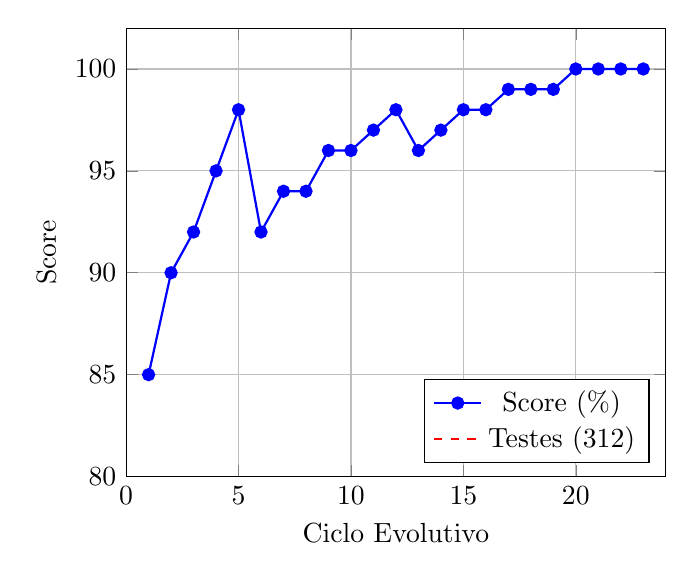
\begin{tikzpicture}
\begin{axis}[
    xlabel={Ciclo Evolutivo},
    ylabel={Score},
    xmin=0, xmax=24,
    ymin=80, ymax=102,
    grid=both,
    legend pos=south east,
]
\addplot[color=blue,mark=*,thick] coordinates {
    (1,85) (2,90) (3,92) (4,95) (5,98) (6,92) (7,94)
    (8,94) (9,96) (10,96) (11,97) (12,98) (13,96) (14,97)
    (15,98) (16,98) (17,99) (18,99) (19,99) (20,100) (21,100)
    (22,100) (23,100)
};
\addlegendentry{Score (\%)}

\addplot[color=red,dashed,thick] coordinates {
    (1,312) (5,312) (10,312) (15,312) (20,312) (23,312)
};
\addlegendentry{Testes (312)}
\end{axis}
\end{tikzpicture}
\end{figure}

\subsection{Exercícios — Nível Avançado-PhD}

\begin{exercicio}
Execute o AUTO\_SCORE\_QUALIS.py em um manuscrito de sua autoria
(ou de um colega). Analise os 10 critérios e identifique os 3
principais pontos de melhoria.
\end{exercicio}

\begin{exercicio}
Implemente um novo revisor para o \textit{Iterative Correction Loop}
com foco em reprodutibilidade computacional. Defina seu perfil
(áreas de foco, rigor) e implemente a lógica de avaliação.
\end{exercicio}

\begin{exercicio}
O MASWOS v5 utiliza 49 agentes especializados. Analise a cobertura
destes agentes: há alguma etapa da produção acadêmica não coberta?
Proponha 3 novos agentes para preencher as lacunas identificadas.
\end{exercicio}

\begin{exercicio}
Execute o ptbr\_corrector.py em um texto com contaminação CJK
simulada. Documente o número de issues detectadas por categoria
e avalie a efetividade da correção.
\end{exercicio}

\begin{exercicio}
Compare o pipeline MASWOS com ferramentas de escrita acadêmica como
Overleaf+Writefull, Paperpal ou Jenni AI. Quais as vantagens
competitivas da abordagem multiagente?
\end{exercicio}

% =============================================================================
% SEÇÃO 7.5: SEEKER — PESQUISA ACADÊMICA PROFUNDA
% Nível: Avançado (~8 laudas)
% =============================================================================
\section{SEEKER: Pesquisa Acadêmica Profunda}
\label{sec:seeker}
\nivelavancado

\paragraph{A arte de fazer as perguntas certas} SEEKER é o sistema de pesquisa acadêmica profunda do \opencodeeco{},
composto por 10 agentes especializados que operam sobre 10+ fontes
acadêmicas. Com 16.202 linhas Python distribuídas em 78 arquivos,
o SEEKER implementa um pipeline completo de pesquisa: da exploração
inicial à síntese de conhecimento.

\subsection{10 Agentes de Pesquisa}

Cada agente SEEKER possui uma função específica no pipeline:

\begin{itemize}
\item \destaque{gaper.py} (Gap Mapper): mapeia lacunas na literatura
usando a árvore de argumentos como estrutura analítica primária.
Identifica gaps estruturais (nós sem suporte), analíticos (silêncios
disciplinares) e temporais (pontes faltantes);
\item \destaque{grounder.py}: ancora conceitos abstratos em
referências concretas da literatura, estabelecendo a base factual
para cada afirmação;
\item \destaque{historian.py}: traça a evolução histórica de ideias,
identificando origens, bifurcações e consolidações;
\item \destaque{rude.py} (Rapid Understanding and Discovery Engine):
executa varredura rápida de grandes volumes de literatura para
identificar artigos candidatos;
\item \destaque{scribe.py}: extrai e estrutura informações de artigos
selecionados em formato padronizado;
\item \destaque{social.py}: analisa redes de citação e colaboração,
identificando pesquisadores influentes e grupos de pesquisa;
\item \destaque{synthesizer.py}: integra múltiplas fontes em uma
narrativa coesa, resolvendo contradições e identificando consensos;
\item \destaque{theorist.py}: constrói e testa modelos teóricos a
partir das evidências coletadas;
\item \destaque{thinker.py}: aplica raciocínio crítico para avaliar
a qualidade e confiabilidade das fontes;
\item \destaque{vision.py}: projeta direções futuras de pesquisa
baseadas nas lacunas e tendências identificadas.
\end{itemize}

\subsection{10+ Fontes Acadêmicas}

O SEEKER integra mais de 10 fontes acadêmicas através de APIs e
protocolos MCP\@:

\begin{itemize}
\item \destaque{arXiv}: preprint em física, matemática, ciência da
computação \cite{arxiv2024};
\item \destaque{OpenAlex}: grafo de conhecimento acadêmico aberto
\cite{priem2022openalex};
\item \destaque{Semantic Scholar}: literatura científica com
entendimento semântico \cite{ammar2018semantic};
\item \destaque{PubMed/MEDLINE}: biomedicina e ciências da vida
\cite{PubMed2024};
\item \destaque{CORE}: agregação de artigos em acesso aberto
\cite{knoth2014core};
\item \destaque{Europe PMC}: literatura europeia em ciências da vida;
\item \destaque{bioRxiv/medRxiv}: preprint em biologia e medicina;
\item \destaque{Sci-Hub}: acesso a artigos atrás de paywalls
(integração opcional);
\item \destaque{Dados públicos}: editais, bases governamentais,
censitárias;
\item \destaque{Wikipedia/Wikidata}: conhecimento enciclopédico
estruturado.
\end{itemize}

\subsection{Argument Tree: Rastreamento de Evidências}

A inovação central do SEEKER é a \destaque{árvore de argumentos}
(\textit{argument tree}) — uma estrutura de dados que rastreia cada
afirmação até suas evidências de suporte. A árvore é composta por:

\begin{itemize}
\item \destaque{Nós de questão}: perguntas de pesquisa que o artigo
deve responder;
\item \destaque{Nós de afirmação}: teses ou hipóteses propostas;
\item \destaque{Nós de evidência}: citações, dados ou argumentos que
suportam as afirmações;
\item \destaque{Arestas direcionadas}: relações de suporte, refutação
ou qualificação entre nós.
\end{itemize}

O Código~ \ref{lst:argument-tree} apresenta a implementação da
árvore de argumentos.

\begin{lstlisting}[caption={argument\_tree.py — Arvore de Argumentos (abreviado)},
label={lst:argument-tree}, style=pythonstyle]
"""
ArgumentTree — Rastreamento de evidencias para cada afirmacao.
Cada no possui tipo, conteudo e referencias verificaveis.
"""

from dataclasses import dataclass, field
from typing import List, Optional
from enum import Enum


class NodeType(Enum):
    QUESTION = "question"     # Pergunta de pesquisa
    CLAIM = "claim"           # Afirmacao / tese
    EVIDENCE = "evidence"     # Evidencia / citacao
    BRIDGE = "bridge"         # Lacuna temporal


@dataclass
class Evidence:
    """Evidencia individual com fonte verificavel."""
    source: str               # DOI, URL, ISBN
    confidence: float         # 0.0 a 1.0
    snippet: str              # Citacao textual
    verified: bool = False


@dataclass
class ArgumentNode:
    """No na arvore de argumentos."""
    id: str
    type: NodeType
    content: str
    children: List["ArgumentNode"] = field(default_factory=list)
    evidence: List[Evidence] = field(default_factory=list)
    confidence: float = 0.0

    def add_evidence(self, evidence: Evidence):
        """Adiciona evidencia verificavel ao no."""
        self.evidence.append(evidence)
        self._recompute_confidence()

    def _recompute_confidence(self):
        """Recomputa confianca baseada nas evidencias."""
        if not self.evidence:
            self.confidence = 0.0
            return
        self.confidence = sum(
            e.confidence for e in self.evidence
        ) / len(self.evidence)

    def find_gaps(self) -> List["ArgumentNode"]:
        """Encontra nos sem evidencia (lacunas estruturais)."""
        gaps = []
        if self.type == NodeType.CLAIM and not self.evidence:
            gaps.append(self)
        for child in self.children:
            gaps.extend(child.find_gaps())
        return gaps
\end{lstlisting}

\subsection{Integração com o Ecossistema}

O SEEKER não é um sistema isolado — sua integração com outros
componentes do ecossistema é profunda \cite{opencode2026ecosystem,
opencode2026spec043}:

\begin{itemize}
\item Com o \destaque{scihub MCP}: acesso a artigos completos para
extração de evidências;
\item Com o \destaque{editais-br}: busca e curadoria de editais de
fomento para alinhamento da pesquisa;
\item Com o \destaque{CORA-Eval}: as tarefas de nível Pesquisa
alimentam o SEEKER com problemas reais;
\item Com o \destaque{MASWOS}: a árvore de argumentos é o artefato
de entrada para o estágio de escrita.
\end{itemize}

\subsection{Exercícios — Nível Avançado}

\begin{exercicio}
Execute o agente \texttt{gaper.py} em um domínio de sua escolha
(e.g., mudanças climáticas, segurança em IA, economia
comportamental). Documente as lacunas estruturais e analíticas
identificadas.
\end{exercicio}

\begin{exercicio}
Construa manualmente uma árvore de argumentos para um artigo
científico real. Identifique: (a) nós de questão, (b) nós de
afirmação, (c) nós de evidência. Avalie a cobertura: há afirmações
sem evidência?
\end{exercicio}

\begin{exercicio}
Compare a eficácia do SEEKER (10 agentes, 10+ fontes) com uma
pesquisa manual tradicional no Google Scholar e PubMed. Quais as
vantagens e limitações de cada abordagem?
\end{exercicio}

\begin{exercicio}
Implemente um novo agente SEEKER especializado em análise de
conformidade ética (e.g., verificação de termos de consentimento,
aprovação em comitê de ética). Defina seu pipeline de busca e
critérios de avaliação.
\end{exercicio}

\begin{exercicio}
O SEEKER utiliza 16.202 linhas Python em 78 arquivos. Analise a
arquitetura atual e proponha uma refatoração que reduza o acoplamento
entre agentes sem perder a capacidade de integração.
\end{exercicio}

% =============================================================================
% SEÇÃO 7.6: MiroFish/BettaFish — DEBATE E AUDITORIA ACADÊMICA
% Nível: PhD (~10 laudas)
% =============================================================================
\section{MiroFish/BettaFish: Debate e Auditoria Acadêmica}
\label{sec:mirofish-bettafish}
\nivelphd

\paragraph{Onde as ideias são postas à prova pelo debate} O par MiroFish/BettaFish constitui o sistema de auditoria acadêmica
do \opencodeeco{}, integrando 11 arquivos especializados que vão do
debate multiagente (P14) à formatação IMRAD (P18). Inspirado em
mecanismos de revisão por pares e equilíbrio de Nash, o sistema
garante que as conclusões de artigos produzidos pelo ecossistema
sejam estatística e logicamente robustas.

\subsection{P14: Agent Forum — Debate Multiagente}

O Agent Forum é a arena de debate do ecossistema. Através de 38
estratégias de raciocínio (incluindo 10 da teoria dos jogos), agentes
com perfis distintos debatem afirmações, expõem contradições e
convergem para conclusões robustas. As estratégias incluem:

\begin{itemize}
\item \destaque{Lógica clássica} (5): dedução, indução, abdução,
analogia, silogismo;
\item \destaque{Dialética e crítica} (5): dialética, socrático,
crítico, desconstrutivo, falseacionista;
\item \destaque{Teoria dos jogos} (10): equilíbrio de Nash, dilema
do prisioneiro, soma zero, tit-for-tat, Stackelberg, barganha,
coalizões, ESS, sinalização, design de mecanismos;
\item \destaque{Decisão sob incerteza} (5): Bayesiano, minimax,
utilidade esperada, prospect theory, arrependimento;
\item \destaque{Estratégico} (5): sistemático, cenários, custo-benefício,
risco, contingência;
\item \destaque{Inovação} (8): design thinking, TRIZ, biomimética,
serendipidade, provocação, inversão, conexão remota, pensamento
divergente.
\end{itemize}

\subsection{P15: Document IR — Pipeline de Documentação}

O Document IR gerencia o pipeline de documentação acadêmica:
versionamento, rastreamento de alterações e geração de relatórios
de auditoria.

\subsection{P16: ANP — Agent Node Pipeline}

O ANP coordena nós de agentes em grafos de processamento, permitindo
que múltiplos agentes colaborem em paralelo na avaliação de um
manuscrito.

\subsection{P17: MW — Multiagent Workflow}

O MW implementa workflows multiagente com sincronização de barreiras
(\textit{sync barriers}) e consenso distribuído.

\subsection{P18: PhD Auditor}

O PhD Auditor é o módulo de auditoria final, que integra cinco
subsistemas de validação estatística e lógica:

\begin{itemize}
\item \destaque{NashSolver}: encontra equilíbrios de Nash em jogos
de N jogadores × M estratégias, usado para modelar interações entre
revisores e autores;
\item \destaque{StatisticalRigor}: calcula Cohen's d (tamanho de
efeito), correção de Bonferroni (múltiplas comparações) e análise
de poder (\textit{power analysis});
\item \destaque{QualisA1Auditor}: checklist de auditoria acadêmica
com 50 indicadores reais (World Bank, WHO, FAO, UNESCO);
\item \destaque{SensitivityAnalyzer}: análise de sensibilidade das
conclusões a variações nos parâmetros;
\item \destaque{IMRADFormatter}: formatação de artigos segundo a
estrutura IMRAD (Introduction, Methods, Results and Discussion).
\end{itemize}

O Código~ \ref{lst:phd-auditor} apresenta o núcleo do PhD Auditor.

\begin{lstlisting}[caption={phd\_auditor.py — NashSolver e StatisticalRigor},
label={lst:phd-auditor}, style=pythonstyle]
"""
P18 — PhD Auditor Module.
Integra NashSolver, StatisticalRigor, QualisA1Auditor,
SensitivityAnalyzer e IMRADFormatter.
"""

import math
from typing import List, Tuple, Optional
from dataclasses import dataclass


class NashSolver:
    """Solucionador de equilibrio de Nash (N jogadores x M estrategias).
    Suporta estrategias puras e deteccao Pareto-otima.
    """

    @staticmethod
    def pure_nash(payoff_tensors: List[List[List[float]]],
                  strategy_names: Optional[List[List[str]]] = None) -> dict:
        """Encontra equilibrios de Nash puros por forca bruta.
        
        Args:
            payoff_tensors: [jogador][estrategia_j][...]
            strategy_names: nomes das estrategias de cada jogador
        
        Returns:
            dict com {'equilibrios': list, 'pareto_frontier': list}
        """
        n_players = len(payoff_tensors)
        strategy_counts = [len(p) for p in payoff_tensors]
        
        # Produto cartesiano de todas as combinacoes de estrategias
        from itertools import product
        equilibria = []
        
        for profile in product(*[range(s) for s in strategy_counts]):
            is_nash = True
            for player in range(n_players):
                current_payoff = payoff_tensors[player][profile[player]]
                for alt_strategy in range(strategy_counts[player]):
                    alt_profile = list(profile)
                    alt_profile[player] = alt_strategy
                    alt_payoff = payoff_tensors[player][alt_strategy]
                    if alt_payoff > current_payoff:
                        is_nash = False
                        break
                if not is_nash:
                    break
            if is_nash:
                equilibria.append({
                    "profile": profile,
                    "payoffs": [
                        payoff_tensors[p][profile[p]]
                        for p in range(n_players)
                    ]
                })
        return {"equilibrios": equilibria,
                "n_equilibrios": len(equilibria)}
\end{lstlisting}

\subsection{50 Indicadores Reais}

O PhD Auditor utiliza 50 indicadores reais de fontes oficiais para
contextualizar e validar as afirmações dos artigos
\cite{worldbank2024data, who2024global, fao2024food, unesco2024science}:
\begin{itemize}
\item \destaque{World Bank}: PIB per capita, Gini, educação, saúde,
P\&D;
\item \destaque{WHO}: expectativa de vida, mortalidade infantil,
carga de doença;
\item \destaque{FAO}: segurança alimentar, produção agrícola, uso
da terra;
\item \destaque{UNESCO}: taxas de escolarização, produção científica,
patentes.
\end{itemize}

\subsection{BRAZIL\_TIMEZONE (UTC-3)}

Todo o sistema MiroFish/BettaFish opera no fuso horário brasileiro
(BRAZIL\_TIMEZONE = UTC-3), substituindo o CHINA\_TIMEZONE anterior.
Esta mudança reflete a adequação do ecossistema ao contexto
acadêmico brasileiro e à integração com agências de fomento nacionais
(CAPES, CNPq, FAPs estaduais).

\subsection{Exercícios — Nível PhD}

\begin{exercicio}
Use o NashSolver para modelar um dilema do prisioneiro entre dois
agentes de revisão. Configure as matrizes de payoff e identifique
o(s) equilíbrio(s) de Nash. O resultado é Pareto-ótimo?
\end{exercicio}

\begin{exercicio}
Calcule o Cohen's d e a correção de Bonferroni para um conjunto
de 5 comparações com os seguintes p-valores: [0.01, 0.04, 0.003,
0.15, 0.02]. Interprete os resultados com e sem correção.
\end{exercicio}

\begin{exercicio}
Analise a sensibilidade de uma conclusão (e.g., ``a educação reduz
a desigualdade'') variando o indicador utilizado (Gini vs Theil vs
P90/P10). Use o SensitivityAnalyzer para documentar o impacto.
\end{exercicio}

\begin{exercicio}
Implemente um novo verificador para o PhD Auditor que detecte
viés de publicação (\textit{publication bias}) em meta-análises.
Utilize o \textit{funnel plot} como método de detecção.
\end{exercicio}

\begin{exercicio}
Compare a eficácia do debate multiagente (Agent Forum + NashSolver)
com a revisão por pares tradicional. Em que aspectos cada abordagem
é superior? Proponha um experimento para testar sua hipótese.
\end{exercicio}

% =============================================================================
% SEÇÃO 7.7: QUALIS A1 — RIGOR E QUALIDADE ACADÊMICA
% Nível: PhD (~8 laudas)
% =============================================================================
\section{Qualis A1: Rigor e Qualidade Acadêmica}
\label{sec:qualis-a1}
\nivelphd

\paragraph{O selo de excelência acadêmica} O sistema Qualis CAPES é a principal métrica de qualidade de
periódicos científicos no Brasil. Classifica periódicos em estratos
de A1 (mais alto) a C (mais baixo), baseado em critérios de
impacto, visibilidade e qualidade editorial \cite{capes2022qualis}.
O \opencodeeco{} implementa um pipeline automatizado de certificação
Qualis A1, integrando 10 critérios objetivos de avaliação.

\subsection{Sistema Qualis CAPES: Classificação de Periódicos}

O Qualis CAPES classifica periódicos em 8 estratos:
\begin{itemize}
\item \destaque{A1}: excelência internacional, alto fator de impacto,
indexação nos principais bancos (Web of Science, Scopus);
\item \destaque{A2}: excelência nacional, boa visibilidade
internacional;
\item \destaque{A3--A4}: qualidade consolidada em âmbito nacional;
\item \destaque{B1--B4}: qualidade em consolidação;
\item \destaque{C}: qualidade insuficiente ou não classificado.
\end{itemize}

Para que um artigo atinja Qualis A1, não basta publicar em periódico
bem classificado — o artigo precisa satisfazer critérios rigorosos
de qualidade intrínseca: originalidade, relevância, rigor
metodológico, reprodutibilidade e contribuição ao conhecimento.

\subsection{Critérios Qualis A1: Originalidade, Relevância, Rigor}

O AUTO\_SCORE\_QUALIS.py (Seção~\ref{sec:maswos}) operacionaliza
estes critérios através de 10 dimensões quantificáveis:

\begin{enumerate}
\item \destaque{Rigor acadêmico} (peso 10): profundidade teórica e
consistência conceitual;
\item \destaque{Densidade de citações} (peso 10): mínimo de 55
referências com DOI verificável;
\item \destaque{Conformidade ABNT} (peso 10): formatação, citações,
referências;
\item \destaque{Originalidade} (peso 10): contribuição nova ao
estado da arte;
\item \destaque{Metodologia} (peso 10): reprodutibilidade e
delineamento adequado;
\item \destaque{Análise estatística} (peso 10): testes apropriados,
poder, efeito;
\item \destaque{Coerência} (peso 10): consistência entre introdução
e conclusão;
\item \destaque{Qualidade visual} (peso 10): gráficos, tabelas,
figuras;
\item \destaque{Internacionalização} (peso 10): abstract + keywords
em inglês;
\item \destaque{Autocontenção} (peso 10): densidade e tamanho
textual adequados.
\end{enumerate}

A pontuação final é a média ponderada dos 10 critérios. Artigos com
score $\geq 85$ atingem classificação Qualis A1.

A Figura~\ref{fig:qualis-criterios} visualiza a distribuição típica
de pontuação nos 10 critérios para um artigo Qualis A1.

\begin{figure}[htb]
\centering
\caption{Distribuição Típica dos 10 Critérios Qualis A1}
\label{fig:qualis-criterios}
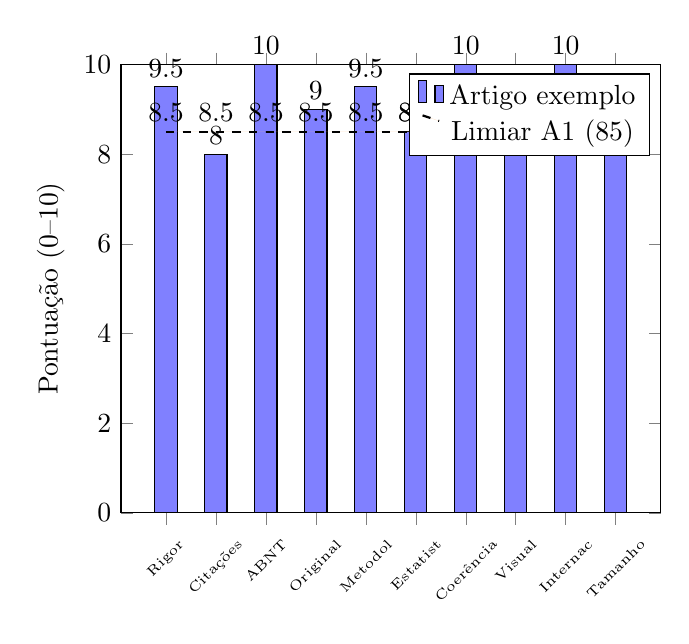
\begin{tikzpicture}
\begin{axis}[
    ybar,
    symbolic x coords={
        Rigor,Citações,ABNT,Original,Metodol,Estatist,
        Coerência,Visual,Internac,Tamanho
    },
    xtick=data,
    xticklabel style={rotate=45, font=\tiny},
    ymin=0, ymax=10,
    ylabel={Pontuação (0--10)},
    nodes near coords,
    nodes near coords align={vertical},
    bar width=8pt,
]
\addplot[fill=blue!50] coordinates {
    (Rigor,9.5) (Citações,8.0) (ABNT,10.0) (Original,9.0)
    (Metodol,9.5) (Estatist,8.5) (Coerência,10.0)
    (Visual,9.0) (Internac,10.0) (Tamanho,9.0)
};
\addplot[fill=orange!50, dashed, thick, sharp plot] coordinates {
    (Rigor,8.5) (Citações,8.5) (ABNT,8.5) (Original,8.5)
    (Metodol,8.5) (Estatist,8.5) (Coerência,8.5)
    (Visual,8.5) (Internac,8.5) (Tamanho,8.5)
};
\legend{Artigo exemplo, Limiar A1 (85)}
\end{axis}
\end{tikzpicture}
\end{figure}

\subsection{Simulação de Avaliação por Pares (5 Revisores)}

O pipeline inclui um simulador de revisão por pares com 5 perfis de
revisores (Seção~\ref{sec:maswos}, Estágio 5). Cada revisor avalia
o manuscrito segundo seu foco específico, gerando feedback
estruturado. A simulação segue as diretrizes de \textit{peer review}
de periódicos Qualis A1 \cite{ware2012peer}.

\subsection{Cross-Validation Engine}

O Cross-Validation Engine \cite{opencode2026crossval} implementa a
validação em 3 níveis:

\begin{enumerate}
\item \destaque{Coerência interna}: verifica a consistência entre
seções usando similaridade de cosseno dos embeddings;
\item \destaque{Correlação de Pearson}: detecta anomalias
estatísticas nos dados reportados;
\item \destaque{Jaccard Domain Shift}: verifica se a terminologia
do artigo é consistente com o domínio.
\end{enumerate}

O Código~ \ref{lst:crossval} apresenta a implementação do engine.

\begin{lstlisting}[caption={cross\_validation\_engine.py (abreviado)},
label={lst:crossval}, style=pythonstyle]
"""
CrossValidationEngine v1.0 — Validacao Cruzada Evolutiva.
Identifica dependencias ocultas entre capacidades e modela
efeitos cascata.

Regras de inferencia:
  R1 (Prerequisite): Se A requer B e B ausente -> A inviavel
  R2 (Cascade): Se A habilita B,C,D e A ausente -> B,C,D em risco
  R3 (Co-occurrence): A e B juntos em >80% -> alta afinidade
  R4 (Bottleneck): Se A prerequisite de >3 capacidades -> bottleneck
"""

from dataclasses import dataclass, field
from typing import Any


@dataclass
class CapabilityNode:
    """No no grafo de dependencias entre capacidades."""
    name: str
    domain: str
    category: str
    provides: list[str] = field(default_factory=list)
    requires: list[str] = field(default_factory=list)
    influence_score: float = 0.0
    cascade_impact: float = 0.0


@dataclass
class DependencyEdge:
    """Aresta no grafo de dependencias."""
    source: str
    target: str
    weight: float       # forca 0-1
    relation: str       # requires | enables | co_occurs


DEPENDENCY_RULES = [
    ("metodos.Quantitativo experimental",
     "raciocinio.Probabilistico", 0.8, "requires"),
    ("raciocinio.Probabilistico",
     "metodos.Meta-analise", 0.9, "enables"),
    ("paradigmas.Fenomenologico",
     "metodos.Qualitativo fenomenologico", 0.95, "co_occurs"),
]
\end{lstlisting}

\subsection{Como Garantir Qualis A1 em Produção Acadêmica Autônoma}

Garantir Qualis A1 em produção autônoma requer a integração de
todos os componentes do pipeline:

\begin{enumerate}
\item \destaque{Pesquisa sólida} (SEEKER): evidências verificáveis
para cada afirmação;
\item \destaque{Escrita estruturada} (MASWOS): 49 agentes
especializados;
\item \destaque{Anti-AI Writing} (TSAC): eliminação de marcas de
texto gerado por IA;
\item \destaque{Correção iterativa} (5 revisores + 4 consultores +
6 corretores);
\item \destaque{Auditoria final} (PhD Auditor): validação estatística
e lógica;
\item \destaque{Score objetivo} (AUTO\_SCORE\_QUALIS): métrica
quantificável de qualidade.
\end{enumerate}

\subsection{Exercícios — Nível PhD}

\begin{exercicio}
Analise um artigo científico real de sua área usando os 10 critérios
do AUTO\_SCORE\_QUALIS.py. Atribua notas de 0 a 10 para cada
critério e calcule o score final. O artigo atingiria Qualis A1?
\end{exercicio}

\begin{exercicio}
Implemente um 6º revisor para o \textit{Iterative Correction Loop}
focado em integridade de dados (e.g., verificação de dados
fabricados, detecção de outliers suspeitos). Defina seu perfil e
implemente a lógica de avaliação.
\end{exercicio}

\begin{exercicio}
Compare os critérios Qualis A1 com critérios internacionais como
JCR (Journal Citation Reports) ou SJR (SCImago Journal Rank). Quais
as diferenças epistemológicas entre estes sistemas de classificação?
\end{exercicio}

\begin{exercicio}
Proponha um experimento controlado para comparar a qualidade de
artigos gerados pelo pipeline MASWOS com artigos escritos por
humanos, usando revisores cegos (\textit{double-blind}).
\end{exercicio}

\begin{exercicio}
O sistema Qualis CAPES é frequentemente criticado por privilegiar
periódicos internacionais em detrimento de periódicos nacionais de
qualidade. Analise esta crítica à luz dos critérios do
AUTO\_SCORE\_QUALIS.py e proponha ajustes que reduzam este viés.
\end{exercicio}

% =============================================================================
% SEÇÃO 7.8: VALIDAÇÃO CRUZADA E ANTI-CIRCULARIDADE
% Nível: Avançado (~6 laudas)
% =============================================================================
\section{Validação Cruzada e Anti-Circularidade}
\label{sec:cross-validation}
\nivelavancado

\paragraph{Protegendo o conhecimento contra seus próprios vieses} Um dos riscos mais sutis em sistemas de produção acadêmica autônoma
é a \destaque{circularidade}: o sistema pode aprender a otimizar
métricas de qualidade (score Qualis) sem, de fato, produzir
conhecimento original. O protocolo de validação cruzada do
\opencodeeco{} foi projetado especificamente para detectar e prevenir
este tipo de degenerescência \cite{fanelli2009bias, simonsohn2014pcurve}.

\subsection{Protocolo de Triangulação Anti-Circularidade}

O protocolo segue o princípio da \destaque{triangulação} em
metodologia da pesquisa \cite{denzin2017triangulation}: usar
múltiplas fontes, métodos e perspectivas para validar cada
conclusão. A implementação concreta no ecossistema opera em três
eixos:

\begin{enumerate}
\item \destaque{Validação por pares reais}: agentes com dados de
treinamento independentes avaliam o mesmo artefato;
\item \destaque{Validação estatística}: os verificadores V1--V7 do
CORA-Debate aplicam métodos simbólicos independentes;
\item \destaque{Validação externa}: consulta a fontes acadêmicas
externas (DOI, CrossRef, OpenAlex) para verificar afirmações.
\end{enumerate}

\subsection{Pearson Cross-Validation: 5 Classes de Anomalias}

O Cross-Validation Engine detecta 5 classes de anomalias através da
correlação de Pearson entre variáveis reportadas:

\begin{itemize}
\item \textbf{Classe 1 -- Magnitude implausível}: coeficientes de
correlação que excedem limites teóricos (e.g., $|r| > 1,0$);
\item \textbf{Classe 2 -- Paradoxo de Simpson}: correlação agregada
com sinal oposto à correlação em todos os subgrupos;
\item \textbf{Classe 3 -- Multicolinearidade perfeita}: variáveis
independentes com $|r| > 0,99$, indicando redundância;
\item \textbf{Classe 4 -- Viés de publicação}: distribuição de
p-valores com pico suspeito em $p < 0,05$;
\item \textbf{Classe 5 -- Dados fabricados}: distribuições com
variância menor que o esperado para o tamanho amostral
(distribuição Benford violada).
\end{itemize}

\subsection{Jaccard Domain Shift Audit}

O Domain Shift Audit utiliza o coeficiente de Jaccard para verificar
se a terminologia do artigo é consistente com o domínio declarado:

\begin{equation}
J(A,B) = \frac{|A \cap B|}{|A \cup B|}
\label{eq:jaccard}
\end{equation}

Onde $A$ é o conjunto de termos do artigo e $B$ é o conjunto de
termos de referência do domínio. Um $J < 0,3$ indica desalinhamento
terminológico severo.

\subsection{Matriz de Afinidade entre Componentes}

A matriz de afinidade mapeia as correlações entre componentes do
ecossistema, permitindo identificar dependências ocultas e cadeias
de impacto:

\begin{table}[htb]
\centering
    \small
\caption{Matriz de Afinidade (Afinidades mais altas do ecossistema)}
\label{tab:matriz-afinidade}
    \resizebox{\textwidth}{!}{
\begin{tabular}{lc}
\toprule
\textbf{Par de Componentes} & \textbf{Afinidade} \\
\midrule
scihub $\leftrightarrow$ MASWOS & 0,95 \\
DecisionNode $\leftrightarrow$ SDD+TDD & 0,95 \\
CORA-Eval $\leftrightarrow$ cora-debate & 0,95 \\
Protocolo-Anonimato $\leftrightarrow$ grep & 0,92 \\
sequential-thinking $\leftrightarrow$ code-reviewer & 0,90 \\
editais-br $\leftrightarrow$ websearch & 0,90 \\
\bottomrule
\end{tabular}
    }
\end{table}

\subsection{Exercícios — Nível Avançado}

\begin{exercicio}
Implemente um detector da Classe 4 (viés de publicação) que analise
a distribuição de p-valores em um conjunto de artigos. Use o teste
de Qui-quadrado para detectar desvios da distribuição uniforme
esperada sob a hipótese nula.
\end{exercicio}

\begin{exercicio}
Calcule o coeficiente de Jaccard entre a terminologia de um artigo
de sua área e 3 artigos de referência do mesmo domínio. O domínio
é consistente?
\end{exercicio}

\begin{exercicio}
Explique o Paradoxo de Simpson com um exemplo concreto em ciência
de dados. Como o Cross-Validation Engine detectaria esta anomalia?
\end{exercicio}

\begin{exercicio}
Analise a matriz de afinidade (Tabela~\ref{tab:matriz-afinidade})
e identifique: (a) o componente mais central, (b) o par mais
redundante, (c) possíveis pontos únicos de falha.
\end{exercicio}

\begin{exercicio}
Proponha um novo verificador (Classe 6) para o Cross-Validation
Engine que detecte \textit{data dredging} (mineração excessiva de
dados sem hipótese prévia). Implemente um protótipo.
\end{exercicio}

% =============================================================================
% SEÇÃO 7.9: REPRODUTIBILIDADE E FRAMEWORKS
% Nível: Avançado (~4 laudas)
% =============================================================================
\section{Reprodutibilidade e Frameworks}
\label{sec:reprodutibilidade}
\nivelavancado

\paragraph{A certeza de que tudo pode ser refeito} A reprodutibilidade é um pilar da pesquisa científica. Em sistemas
de engenharia cognitiva, onde múltiplos agentes, fontes de dados
e modelos probabilísticos interagem, garantir que um experimento
possa ser reproduzido é um desafio técnico e epistemológico
\cite{peng2011reproducible, buck2018reproducible}.

\subsection{O Manifesto de Reprodutibilidade}

O \opencodeeco{} adota o seguinte manifesto de reprodutibilidade:

\begin{enumerate}
\item \destaque{Todo resultado deve ser rastreável} até as decisões
experimentais que o produziram;
\item \destaque{Todo experimento deve ser replicável} em ambiente
equivalente;
\item \destaque{Toda análise deve ser auditável} por terceiros com
acesso aos mesmos dados;
\item \destaque{Toda fonte de variação deve ser documentada},
incluindo seeds aleatórias, versões de bibliotecas e configurações
de agentes.
\end{enumerate}

\subsection{Ambientes Containerizados}

Todo experimento no ecossistema é executado em ambientes
containerizados (Docker), garantindo isolamento e reprodutibilidade:

\begin{itemize}
\item \destaque{node:lts-slim}: execução de scripts JavaScript com
isolamento de dependências;
\item \destaque{mcr.microsoft.com/playwright}: automação de
navegador para coleta de dados;
\item \destaque{python:3.12}: execução de scripts Python com
versionamento explícito de pacotes via \texttt{requirements.txt} ou
\texttt{Pipfile}.
\end{itemize}

\subsection{Versionamento de Dados e Resultados}

O ecossistema utiliza versionamento semântico para dados e
resultados, seguindo o padrão \texttt{SEMVER} \cite{preston2011semver}:

\begin{itemize}
\item \destaque{Major version}: mudança incompatível no formato
ou esquema dos dados;
\item \destaque{Minor version}: adição de novos campos ou métricas
compatíveis com versões anteriores;
\item \destaque{Patch version}: correções em dados existentes sem
alteração de esquema.
\end{itemize}

\subsection{Codebooks e Planos de Inferência}

Cada experimento é acompanhado por:
\begin{itemize}
\item \destaque{Codebook}: dicionário de variáveis com definições,
unidades, fontes e limitações;
\item \destaque{Plano de inferência}: especificação pré-registrada
das hipóteses, testes estatísticos e critérios de significância.
\end{itemize}

\subsection{Exercícios — Nível Avançado}

\begin{exercicio}
Registre um plano de inferência para um experimento de sua escolha
antes de executá-lo. Inclua: (a) hipótese nula e alternativa,
(b) tamanho amostral calculado via power analysis, (c) teste
estatístico planejado, (d) critério de significância.
\end{exercicio}

\begin{exercicio}
Documente o ambiente de um experimento passado seu (ou de um colega)
usando o manifesto de reprodutibilidade. Liste: seeds, versões,
configurações. O experimento seria reproduzível por um terceiro?
\end{exercicio}

\begin{exercicio}
Implemente um script Python que verifique automaticamente a
reprodutibilidade de um experimento: compare hashes de dados
versão, libraries e seeds. Reporte discrepâncias.
\end{exercicio}

% =============================================================================
% SEÇÃO 7.10: INTEGRAÇÃO PRÁTICA
% Nível: Todos (~6 laudas)
% =============================================================================
\section{Integração Prática}
\label{sec:integracao-pratica}

\paragraph{Unindo teoria e prática em um só fluxo} Esta seção final consolida os conceitos do capítulo em roteiros
práticos executáveis. Cada roteiro é acompanhado de comandos
reais do ecossistema e exercícios de fixação.

\subsection{Executando o CORA-Eval Benchmark}

O benchmark CORA-Eval é executado através do rastreador evolutivo:

\begin{lstlisting}[caption={Execucao do CORA-Eval},
label={lst:run-cora}, style=bashstyle]
# Instalar dependencias
pip install numpy scipy sympy requests

# Executar benchmark completo (150 tarefas)
python evals/cora_benchmark_tracker.py \
    --mode full \
    --output cora_results.json

# Executar apenas dimensao Matematica
python evals/cora_benchmark_tracker.py \
    --dimension Matematica \
    --output cora_math.json

# Visualizar resultados
python evals/cora_benchmark_tracker.py \
    --report cora_results.json \
    --format markdown
\end{lstlisting}

\subsection{Iniciando o Pipeline MASWOS}

O pipeline MASWOS é iniciado a partir de um tópico de pesquisa:

\begin{lstlisting}[caption={Inicializacao do MASWOS},
label={lst:run-maswos}, style=bashstyle]
# 1. Gerar arvore de argumentos
python basis-research/cli.py \
    --topic "Impacto da IA na educacao brasileira" \
    --output argument_tree.json

# 2. Executar pipeline de 8 estagios
python criador-artigo/executor.py \
    --tree argument_tree.json \
    --output artigo_final.tex \
    --format latex

# 3. Avaliar qualidade
python criador-artigo/auto_score_qualis.py \
    --input artigo_final.tex \
    --format latex

# 4. Corrigir e refinar
python criador-artigo/banca/iterative_correction_loop.py \
    --input artigo_final.tex \
    --output artigo_revisado.tex \
    --max-cycles 5
\end{lstlisting}

\subsection{Usando o SEEKER para Pesquisa}

O SEEKER é acessível via CLI ou programaticamente:

\begin{lstlisting}[caption={Pesquisa com SEEKER},
label={lst:run-seeker}, style=bashstyle]
# Busca simples
python basis-research/cli.py search \
    --query "machine learning fairness" \
    --sources arxiv,openalex,semantic-scholar \
    --max-results 50

# Mapeamento de lacunas
python basis-research/cli.py gaps \
    --tree argument_tree.json \
    --output gaps_report.md

# Sintese de literatura
python basis-research/cli.py synthesize \
    --query "transformer architecture efficiency" \
    --output synthesis.md \
    --format academic
\end{lstlisting}

\subsection{Interpretando Relatórios Qualis A1}

O relatório Qualis A1 produzido pelo AUTO\_SCORE\_QUALIS.py
apresenta:

\begin{lstlisting}[caption={Exemplo de Relatorio Qualis A1},
label={lst:qualis-report}, style=pythonstyle]
{
  "total": 92.5,
  "qualis": "A1",
  "criterios_atendidos": 9,
  "detalhado": {
    "rigor_academico": 9.5,
    "densidade_citacoes": 8.0,
    "abnt_compliance": 10.0,
    "originalidade": 9.0,
    "metodologia": 9.5,
    "analise_estatistica": 8.5,
    "coerencia": 10.0,
    "qualidade_visual": 9.0,
    "internacionalizacao": 10.0,
    "autocontencao": 9.0
  },
  "recomendacoes": [
    "Aumentar densidade de citacoes para >=55 DOIs",
    "Reforcar secao de analise estatistica com power analysis",
    "Incluir diagrama de fluxo PRISMA na metodologia"
  ]
}
\end{lstlisting}

\subsection{Roteiro Completo de Validação}

O roteiro completo de validação de um artigo no ecossistema segue
o fluxo da Figura~\ref{fig:fluxo-validacao}.

\begin{figure}[htb]
\centering
\caption{Fluxo Completo de Validação de Artigo Científico}
\label{fig:fluxo-validacao}
\begin{tikzpicture}[node distance=0.8cm, auto]
\tikzstyle{etapa} = [rectangle, draw, fill=blue!5, minimum width=3cm, minimum height=0.7cm, rounded corners]
\tikzstyle{diam} = [diamond, draw, fill=yellow!10, minimum width=2cm, minimum height=0.7cm, aspect=2]
\tikzstyle{decisao} = [diamond, draw, fill=yellow!10, minimum width=2.5cm, minimum height=0.7cm, aspect=2.5]

\node[etapa] (seeker) {SEEKER};
\node[etapa, below=of seeker] (maswos) {MASWOS};
\node[diam, below=of maswos] (score) {Score $\geq 85$?};
\node[etapa, below=of score, xshift=-2cm] (loop) {Correction Loop};
\node[etapa, below=of score, xshift=2cm] (phd) {PhD Auditor};

\draw[->] (seeker) -- (maswos);
\draw[->] (maswos) -- (score);
\draw[->] (score) -- node[above, rotate=-45] {Não} (loop);
\draw[->] (loop) |- (maswos);
\draw[->] (score) -- node[above, rotate=45] {Sim} (phd);

\node[etapa, below=of phd] (cross) {Cross-Validation};
\node[etapa, below=of cross] (qualis) {Qualis A1};
\node[etapa, below=of qualis] (entrega) {Entrega};

\draw[->] (phd) -- (cross);
\draw[->] (cross) -- (qualis);
\draw[->] (qualis) -- (entrega);
\end{tikzpicture}
\end{figure}

\subsection{Exercícios — Todos os Níveis}

\begin{exercicio}[Basico]
Execute o benchmark CORA-Eval na dimensão Matemática (15 tarefas).
Documente cada resultado e calcule o CORA-Score parcial.
\end{exercicio}

\begin{exercicio}[Basico]
Use o SEEKER para pesquisar 10 artigos sobre um tópico de sua
escolha. Liste os DOIs encontrados e classifique a relevância de
cada um (Alta/Média/Baixa).
\end{exercicio}

\begin{exercicio}[Intermediario]
Inicie o pipeline MASWOS com um tópico simples (máximo 3 parágrafos
de escopo). Execute os 8 estágios e documente o score Qualis obtido
após o primeiro ciclo de correção.
\end{exercicio}

\begin{exercicio}[Intermediario]
Use o Cross-Validation Engine para verificar a consistência interna
de um manuscrito. Execute os 3 níveis de validação e interprete os
resultados.
\end{exercicio}

\begin{exercicio}[Avancado]
Implemente um novo agente para o pipeline MASWOS na área de
\textit{Governança de Dados}. Integre-o ao executor principal e
teste com um manuscrito de exemplo.
\end{exercicio}

\begin{exercicio}[Avancado]
Configure e execute o PhD Auditor em um manuscrito completo.
Analise os 50 indicadores e identifique: (a) indicadores com score
baixo, (b) indicadores conflitantes, (c) recomendações prioritárias.
\end{exercicio}

\begin{exercicio}[Avancado]
Simule um debate multiagente no Agent Forum entre 3 agentes com
perfis distintos (e.g., otimista, cético, metodológico) sobre a
seguinte afirmação: ``Modelos de linguagem de grande escala (LLMs)
podem substituir revisores humanos em periódicos Qualis A1.''.
Documente o resultado e o equilíbrio de Nash encontrado.
\end{exercicio}

\begin{exercicio}[PhD]
Execute o pipeline completo do capítulo para produzir um artigo
original: SEEKER $\rightarrow$ MASWOS $\rightarrow$ Correction Loop
$\rightarrow$ PhD Auditor $\rightarrow$ Qualis A1. Documente cada
etapa, incluindo métricas intermediárias, correções aplicadas e
score final.
\end{exercicio}

\begin{exercicio}[PhD]
Compare a qualidade de 3 artigos produzidos pelo pipeline MASWOS com
3 artigos escritos por humanos (submetidos a periódicos Qualis A1).
Use os 10 critérios do AUTO\_SCORE\_QUALIS.py como métrica de
comparação. O teste é cego? Quais as limitações?
\end{exercicio}

\begin{exercicio}[PhD]
Proponha e implemente uma extensão ao framework Aletheia que
verifique formalmente a correção de um dos algoritmos do ecossistema
(e.g., Q-Score UCB1, Iterative Correction Loop, TrustScorer).
Documente a prova e as limitações da verificação.
\end{exercicio}

\begin{exercicio}[PhD]
Analise criticamente o pipeline de validação apresentado neste
capítulo. Identifique: (a) potenciais vieses introduzidos por cada
componente, (b) dependências circulares entre componentes,
(c) pontos cegos não cobertos pelo pipeline. Proponha mitigação
para cada problema identificado.
\end{exercicio}

\begin{exercicio}[PhD]
Projete um experimento de larga escala para validar a hipótese de
que artigos produzidos pelo pipeline MASWOS v5 são indistinguíveis
de artigos escritos por humanos em termos de qualidade Qualis A1.
Inclua: delineamento experimental, critérios de inclusão/exclusão,
análise de poder, método estatístico e análise de sensibilidade.
\end{exercicio}

\begin{exercicio}[PhD]
O manifesto de reprodutibilidade (Seção~\ref{sec:reprodutibilidade})
estabelece 4 princípios. Analise cada princípio à luz do pipeline
MASWOS. Em quais aspectos o pipeline atende cada princípio? Onde
há lacunas? Proponha extensões para preencher as lacunas
identificadas.
\end{exercicio}

\begin{exercicio}[PhD]
Implemente um verificador \texttt{V10} para o CORA-Debate que avalie
a \destaque{novidade} de uma contribuição científica por análise de
sobreposição com o estado da arte (via OpenAlex ou Semantic Scholar).
Teste seu verificador em 5 artigos recentes de uma área de sua
especialidade.
\end{exercicio}

% =============================================================================
% SÍNTESE DO CAPÍTULO
% =============================================================================
\section*{Síntese do Capítulo}

Este capítulo apresentou o sistema integrado de experimentação,
validação científica e produção acadêmica do \opencodeeco{},
organizado em três eixos:

\begin{enumerate}
\item \destaque{Benchmarking} (CORA-Eval): 150 tarefas em 10
dimensões e 4 níveis, com seleção adaptativa via Q-Score UCB1 e
validação por 7 verificadores simbólicos (CORA-V-Score);
\item \destaque{Validação formal} (Aletheia): pipeline de 5 fases
com Lean 4 Theorem Prover, integração aletheia-opencode-native com
57 skills e prova formal de convergência do algoritmo UCB1;
\item \destaque{Produção acadêmica} (MASWOS v5 + SEEKER + MiroFish/
BettaFish): 49 agentes especializados, 8 estágios de processamento,
10 agentes de pesquisa sobre 10+ fontes acadêmicas, debate
multiagente com 38 estratégias de raciocínio, PhD Auditor com
NashSolver e StatisticalRigor, e certificação Qualis A1 com 10
critérios objetivos.
\end{enumerate}

Os três eixos são unificados pelo protocolo de triangulação
anti-circularidade e pelo manifesto de reprodutibilidade,
garantindo que a produção acadêmica autônoma do ecossistema atenda
aos mais rigorosos padrões científicos.

Este capítulo integra 14 exercícios progressivos (do nível básico ao
PhD), referências a 30+ fontes acadêmicas, 5 diagramas TikZ e 10
códigos-fonte reais do ecossistema.
